%; whizzy chapter
% -initex iniptex -latex platex -format platex -bibtex jbibtex -fmt fmt
% 以上 whizzytex を使用する場合の設定。


%     Tokyo Debian Meeting resources
%     Copyright (C) 2010 Junichi Uekawa

%     This program is free software; you can redistribute it and/or modify
%     it under the terms of the GNU General Public License as published by
%     the Free Software Foundation; either version 2 of the License, or
%     (at your option) any later version.

%     This program is distributed in the hope that it will be useful,
%     but WITHOUT ANY WARRANTY; without even the implied warranty of
%     MERCHANTABILITY or FITNESS FOR A PARTICULAR PURPOSE.  See the
%     GNU General Public License for more details.

%     You should have received a copy of the GNU General Public License
%     along with this program; if not, write to the Free Software
%     Foundation, Inc., 51 Franklin St, Fifth Floor, Boston, MA  02110-1301 USA

%  preview (shell-command (concat "evince " (replace-regexp-in-string "tex$" "pdf"(buffer-file-name)) "&"))
% 画像ファイルを処理するためにはebbを利用してboundingboxを作成。
%(shell-command "cd image201001; ebb *.png")

%%ここからヘッダ開始。

\documentclass[mingoth,a4paper]{jsarticle}
\usepackage{monthlyreport}

% 日付を定義する、毎月変わります。
\newcommand{\debmtgyear}{2010}
\newcommand{\debmtgmonth}{1}
\newcommand{\debmtgdate}{23}
\newcommand{\debmtgnumber}{60}

\begin{document}

\begin{titlepage}
\thispagestyle{empty}

% タイトルページ:編集必要な部分は最初のマクロに飛ばすこと

\vspace*{-2cm}
第\debmtgnumber{}回 東京エリア Debian 勉強会資料

\hspace*{-2.4cm}
\includegraphics[width=210mm]{image200801/2008title.eps}\\
\hfill{}\debmtgyear{}年\debmtgmonth{}月\debmtgdate{}日

\end{titlepage}


\dancersection{Introduction}{上川 純一}

\begin{multicols}{2}
 
 
 今月のDebian勉強会へようこそ。これからDebianの世界にあしを踏み入れると
 いう方も、すでにどっぷりとつかっているという方も、月に一回Debianについ
 て語りませんか?

 Debian勉強会の目的は下記です。

 \begin{itemize}
 \item \underline{Debian Developer} (開発者)の育成。
 \item 日本語での「\underline{開発に関する情報}」を整理してまとめ、アップデートする。
 \item \underline{場}の提供。
 \begin{itemize}
  \item 普段ばらばらな場所にいる人々が face-to-face で出会える場を提供
	する。
  \item Debian のためになることを語る場を提供する。
  \item Debianについて語る場を提供する。
 \end{itemize}
 \end{itemize}		

 Debianの勉強会ということで究極的には参加者全員がDebian Packageをがりがり
 と作るスーパーハッカーになった姿を妄想しています。情報の共有・活用を通し
 て Debianの今後の能動的な展開への土台として、「場」としての空間を提供す
 るのが目的です。

\end{multicols}

\newpage

\begin{minipage}[b]{0.2\hsize}
 \definecolor{titleback}{gray}{0.9}
 \colorbox{titleback}{\rotatebox{90}{\fontsize{80}{80} {\gt デビアン勉強会} }}
\end{minipage}
\begin{minipage}[b]{0.8\hsize}
\hrule
\vspace{2mm}
\hrule
\tableofcontents
\vspace{2mm}
\hrule
\end{minipage}

\dancersection{事前課題}{上川 純一}

今回の事前課題は以下です:

\begin{enumerate}
 \item 今回の BSP への意気込みを熱く語ってください。
\end{enumerate}

この課題に対して提出いただいた内容は以下です。

\begin{prework}{$B$d$^$@(B}
\preworksection{$B:#2s$N(B BSP $B$X$N0U5$9~$_$rG.$/!)8l$C$F$_$k(B}

Primer$B$H(BRC-bug$B%j%9%HFI$_$J$,$i05E]$5$l$D$D$b!"(B

\begin{itemize}
\item $B$b$&!V$$$D=P$k$N$+K\Ev$K=P$k$N$+!W$H$O8@$o$;$J$$!*(B
\item $B$d$C$Q$j!V%^%@!<!)!W$h$j<+J,$G2?$+$7$F=P$kJ}$,$$$$$h$M!*(B
\item $B$d$k$J$i%H%3%H%s=8CfE*$K$d$C$F%a%s%F%J%9%-%k8~>e$b$7$h$&!*(B
\end{itemize}

$B$H$$$&$3$H$G!"(B10$B8D0LD>$9$3$H$rL\I8$K;22C$7$^$9!#(B

$B<B$O!V=i;22C$,$$$-$J$j(BBSP$B$C$FBg>fIW$+!)!d<+J,!W$J$N$G(B
$B1[$($i$l$J$$JI$r$$$^C[$$$F$7$^$C$?46$,L5$-$K$7$bHs$:$G$9$,!"(B
$BLnK>C#@.$N$?$a$;$C$;$H;E9~$s$G$f$-$^$9$G$9!&!&!&(B

\end{prework}

\begin{prework}{$B2,It(B $B5f(B}
\preworksection{$B:#2s$N(B BSP $B$X$N0U5$9~$_$rG.$/8l$C$F$/$@$5$$(B}
$B$^$:$O<j;}$A$N%Q%C%1!<%8$G$"$k(Buim$B$N(Blintian$B%P%0$r(B0$B$K$7$^$9!#(B
$B$=$N$"$H!"(Buim$B$N%S%k%@$+$i$N%(%i!<Js9p$N2r(B $Bat(B $BO$r$d$j$?$$$H;W$$$^$9!(B?

$B$=$l$G$bM>NO$,$"$C$?$i(Bmlterm$B$N(Blintian$B%P%0$d$=$NB>$N%j%j!<%9%/%j%F%#%+%k(B
$B%P%0$rD>$=$&$H;W$$$^$9!#(B
\end{prework}

\begin{prework}{ $BF|HfLn(B $B7<(B }

groff $B$N%P%0$r<h$k$N$KD)@o$7$F$_$h$&$H;W$$$^$9!#(B

$B$"$H4X?t7?$^$o$j$G2?$+$"$l$P6(NO$7$^$9!#(B

\end{prework}



\begin{prework}{ $BF#BtM}Ao(B(risou) }

$B2?$r$7$?$iNI$$$N$+$bA4A3$o$+$C$F$^$;$s$,!"$3$N5!2q$rMxMQ$7$F!"(BDebian$B$K>/(B
 $B$7$G$b9W8%$G$-$l$P!"$H;W$C$F$$$^$9!#$h$m$7$/$*4j$$$7$^$9!#(B

\end{prework}



\begin{prework}{ kmuto }

$B<+J,$N%Q%C%1!<%8$N%P%0=$@5!"(BRC$B$K8B$i$:;H$C$F$F:$$k%Q%C%1!<%8$N(Bdelay
 upload$B!"$[$+$N?M$N:n6H$N%9%]%s%5!<!"$H$$$C$?$"$?$j$r!#(B
$B;~4|E*$K$A$g$C$HFI$a$J$$$N$G%-%c%s%;%k$9$k$+$b$7$l$^$;$s!#$"$H!";22C$7$F(B
 $B$bESCfB`@J$K$J$k$H;W$$$^$9!#(B


\end{prework}



\begin{prework}{ henrich }

$B<j;}$A$N:n6H$r>/$7$G$b8:$i$7$F$*$3$&$H;W$$$^$9!#(B

\end{prework}



\begin{prework}{ iwamatsu }
RC$B$H(BQA$B$rCf?4$K%P%0$rDY$9M=Dj$G$9!#(B


\end{prework}



\begin{prework}{ $B>e@n=c0l(B }

$B%,%s%,%s%P%0$r$D$V$9M=Dj$G$9!#(B
$B$"$H!"#D#e#b#i#a#nJY6/2qM=Ls%7%9%F%`$K$D$$$F>pJs6&M-$7$?$$$G$9!#(B

\end{prework}


\dancersection{最近のDebian関連のミーティング報告}{前田耕平}
\subsection{東京エリアDebian勉強会59回目報告}
% (query-replace-regexp "<.*?>" "")
% (query-replace-regexp "^[	 ]\+" "")


2010年最後のDebian勉強会は東大駒場キャンパスでの開催でした。

参加者は、あらきさん、キタハラさん、日比野さん、やまねさん、本庄さん、吉田さん、あけどさん、よしのさん、岩松さん、前田の10名でした。

今回はいつもと違い、ワイン飲みながらでの進行。みんなへべれけでした。私はlxcの話をしました。日比野さんに質問されたブリッジの構成の件は、一つ前提条件があったのを忘れていたのでここで補足。
\begin{itemize}
 \item 今回の資料を作るために使っていたサーバは、グローバルIPアドレスではなく、プライベートアドレスを持っている。
 \item インターネットからのアクセスは、ファイアウォールでtcp/80, 22, 443, 5984などの特定ポートのみ、このサーバに宛先NATをしている。
 \item 80, 443, 5984などは、コンテナ上で稼働させているサービスに割り当てたいので、ホストOSで、さらに宛先NATさせている
\end{itemize}

という構成。なので、そもそもコンテナにホストOSと同じブロードキャストドメインのIPアドレスを割り当てる必要はなく、最初から別のセグメントのIPアドレスを割り当てて、宛先NATしておけば、ブリッジ使っているのに宛先NATいらないじゃないか?という疑問は出なかったかもしれません。

他は今年の総括と来年に向けてのディスカッションを岩松さんの仕切りで行われました。in木更津やOSCでのネタ出しで熱いディスカッションができました。まだ送って撮っておいたホワイトボードの写真とかディスカッションしながら更新していた資料をコミット、プッシュしていないのでやっておかないと。

宴会はすでに出来上がった状態で下北沢駅近くの店で鍋でした。ウマー。店の名前は思い出せず。不覚。


%\printindex

\cleartooddpage

\vspace*{15cm}
\hrule
\vspace{2mm}

\includegraphics[width=2cm]{image200502/openlogo-nd.eps}
\noindent \Large \bf Debian 勉強会資料\\ \\
\noindent \normalfont \debmtgyear{}年\debmtgmonth{}月\debmtgdate{}日 \hspace{5mm}  初版第1刷発行\\
\noindent \normalfont 東京エリア Debian 勉強会 (編集・印刷・発行)\\
\hrule

\end{document}
